The website is build to allow exhibition managers to manage their exhibition, as stated in the problem statement \secref{sec:problemstatement}. All concepts of an exhibition can be added from the website, this include feeds, schedule, booths, companies, categories and a floor plan.
The different tabs manage different concepts of an exhibition:


\begin{description}
	\item[Feeds] Here the manager can add a feed to a booth in the database.
	\item[Company] Here the manager can add a company to the database, the company logo will also be uploaded to the server for further use.
	\item[Category] In this tab the manager can add a category to the database for further use.
	\item[Exhib] In the "Exhib" tab the manager can create a new empty exhibition.
	\item[Schedule] In the Schedule tab the manager can create a new schedule and add it to a booth in the database.
	\item[Floor plan] The "floor plan" tab is the heart of the website, here almost all the other concepts can be added, this include, making a new exhibition, complete with a floor plan, categories, companies, and booths. Previous created exhibitions can also be loaded for viewing or editing.
\end{description}


The problem statement \secref{sec:problemstatement} states that booths should be able to create feeds themselves, this have not been used in the design of the website, but it is possible with the integration of a login system on the website. This will also make sure managers only will be able to edit their own exhibitions.


The website is designed with the main focus on the "floor plan" tab, this tab functions almost as a standalone one-page website, though the "feed" and "schedule" tab is also needed to make a "complete" exhibition.


The "floor plan" tab makes use of the Google Maps API, giving a visual presentation when creating an exhibition.
The following steps are required when creating an exhibition floor plan:
\begin{description}
	\item[Step 1] Click the "Create Exhibition" button and fill in the exhibition information.
	\begin{figure}[H]
		\centering
		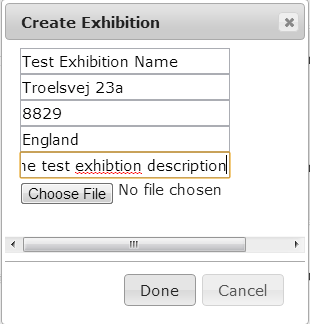
\includegraphics[scale=0.5]{img/website/step2.png}
		\caption{Create exhibition dialogue.\label{fig:websitestep1}}
	\end{figure}
	\item[Step 2] Create a number of markers, which will make up the walking path of the exhibition floor.
	\begin{figure}[H]
		\centering
		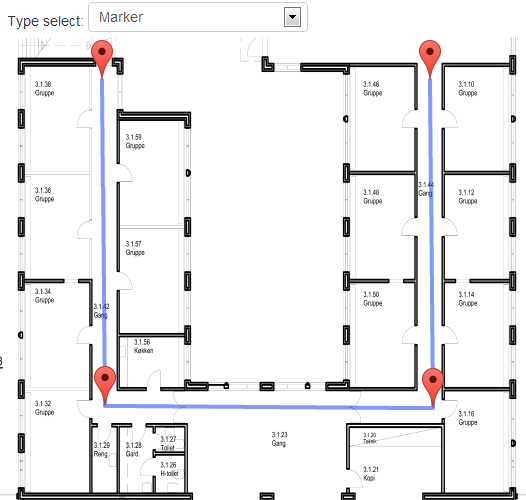
\includegraphics[scale=0.5]{img/website/step3.png}
		\caption{Floor plan walking path.\label{fig:websitestep2}}
	\end{figure}
	\item[Step 3] Create a booth by having selected the "Booth" option, and clicking the floor plan in any given position. When the booth positioning and size is correct, the booth can be locked by clicking it again, this will bring up the "booth information" dialogue. Fill in the booth information, and booth will be saved.
	\begin{figure}[H]
		\centering
		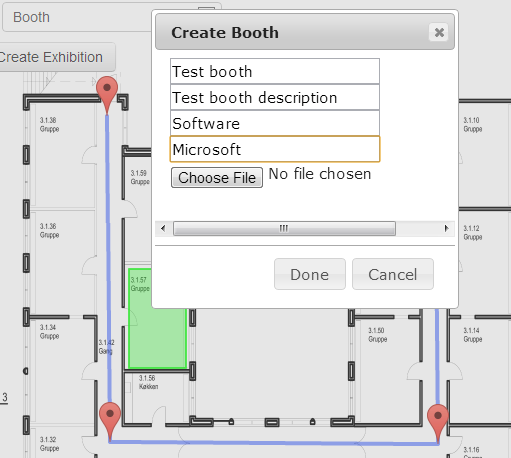
\includegraphics[scale=0.5]{img/website/step4.png}
		\caption{Create booth dialogue.\label{fig:websitestep3}}
	\end{figure}
	\item[Step 4] Repeat step 3, until all booths have been created.
	\item[Step 5] Bind the locked booths by right-clicking them, and then clicking a point on the walking path. This will create a new entry point for the booth.
	\begin{figure}[H]
		\centering
		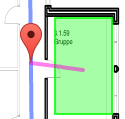
\includegraphics[scale=0.5]{img/website/step5.png}
		\caption{Booth entry point on walking path.\label{fig:websitestep5}}
	\end{figure}
	\item[Step 6] Repeat step 5 until all booths are bound to the walking path, a booth can have multiple entry points.
	\item[Step 7] Save the exhibition by clicking the "Save" button. This will save the exhibition to the database.
\end{description}
For a better overview of creating an floor plan using this feature see \autoref{fig:floorplan}.
\begin{figure}[H]
	\centering
	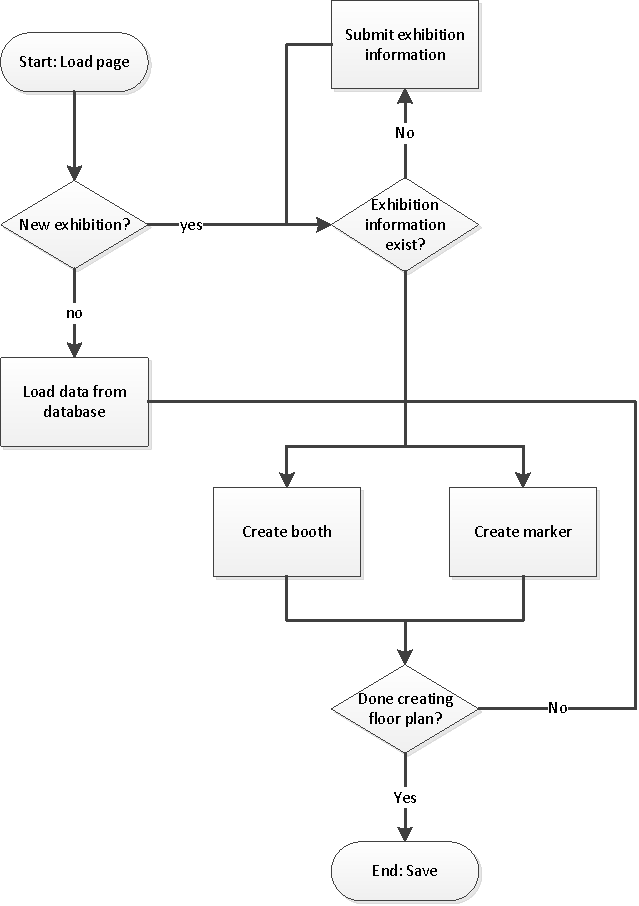
\includegraphics[scale=0.5]{img/floorplanflow.pdf}
	\caption{Flowchart of creating a floor plan.\label{fig:floorplan}}
\end{figure}


After creating an exhibition the user can add feeds to the exhibition, using the "Feeds" tab, feeds are bound to an existing booth from the database. A schedule can be added using the the "schedule" tab, here the user selects a "name", "booth", "start time" and "end time".
It is also possible to load an existing exhibition from the database, for the loaded exhibition the floor plan will be shown on the map. This exhibition can then be edited, and saved to the database, reflecting the changes the user has made.


All form requests on the website is handled using the AJAX technology\citep{ajax}. AJAX is a technique allowing a website to be dynamically updated while the user is looking at it.
The AJAX scripts post form data to PHP, which handles the database interaction. When connecting to the database prepare statements are used, to make sure no malicious data is inserted into the database.


The design of the website is done using Twitter Bootstrap\citep{twitterbootstrap}, a CSS UI supplying a stylish and uniform interface.
The main focus in the website is functionality and therefore the graphic design and usability is not the main priority.